% !TeX root = ../presentation.tex

\section{Data Spaces}

\begin{frame}{Inter-Organisational Information Systems (IOIS) \footnotesize\cite{mollerIndustrialDataEcosystems2024}}
    \begin{columns}
        \begin{column}{0.6\textwidth}
            \begin{itemize}
                \item \alert{bilaterale} Beziehungen, bspw. Lieferketten
                \item tiefe Integration, automatisiertes Data Sharing
                \item zweckgebunden, bspw. Koordinierung und Optimierung von Lieferketten
                % \item Mittel zum Zweck
                \item mangelndes Vertrauen, streng formalisierte Nutzungsrichtlinien
                \item keine Daten teilen? $\to$ Ineffizienz $\to$ Verlust
                \item Herausforderungen bei Skalierung % Datenaustausch, Kontrolle
            \end{itemize}
        \end{column}

        \begin{column}{0.4\textwidth}
            \begin{figure}
                
\includegraphics[height=0.5\textheight]{./assets/iois_architecture.drawio.pdf}
                \caption{IOIS Architektur}
            \end{figure}
        \end{column}
    \end{columns}
\end{frame}


\begin{frame}{Industrial Data Ecosystems \footnotesize\cite{mollerIndustrialDataEcosystems2024}}
    \begin{columns}
        \begin{column}{0.6\textwidth}
            \begin{itemize}
                % \item dynamisch, geteilter Zweck
                \item Gleichgewicht zwischen erhaltenem und gegebenem Aufwand
                \item Daten als strategische Ressource % statt Mittel zum Zweck
                % \item ermöglichen neue Geschäfte und Optimierung von Prozessen
                \item Interaktion und Kooperation \alert{multilateraler} Akteure
                \item Data User, Data Provider, Data Intermediary
                \item offener, dynamischer Datenaustausch
                \item Netzwerkeffekte, Förderung von Innovation
            \end{itemize}
        \end{column}

        \begin{column}{0.4\textwidth}
            \begin{figure}
                \centering
                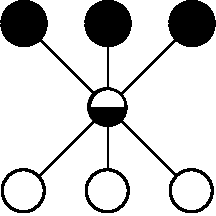
\includegraphics[height=0.5\textheight]{./assets/industrial_de_architecture.drawio.pdf}
                \caption{Industrial Data Ecosystems mit Data Intermediary}
            \end{figure}
        \end{column}
    \end{columns}
\end{frame}


\begin{frame}{Data Spaces \footnotesize\cite{mollerIndustrialDataEcosystems2024}}
    \begin{columns}
        \begin{column}{0.6\textwidth}
            \begin{itemize}
                \item Vereinen von IOIS und Data Intermediaries
                \item dezentrale Speicherung von Daten bei Provider
                \item \emph{Data Space Connectors} für bilateralen Datenaustausch % vgl. IOIS
                \item Zusammenbringen von Data User und Provider % vgl. Data Intermediary
                \item technische Garantie von Datensouveränität % -> Überwindung betriebl. Barrieren
                % \item Kontrolle über Zugriff und Verwendung bei Provider
                \item geteilter Raum für vertrauenswürdiges Data Sharing $\to$ Optimierung, Innovation
            \end{itemize}
        \end{column}

        \begin{column}{0.4\textwidth}
            \begin{figure}
                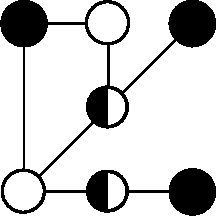
\includegraphics[height=0.5\textheight]{./assets/data_space_architecture.drawio.pdf}
                \caption{Data Space Architektur}
            \end{figure}
        \end{column}
    \end{columns}
\end{frame}


\begin{frame}[c]{Data Spaces II \footnotesize\cite{mollerIndustrialDataEcosystems2024}}
    % verteilt by Design --> Daten bleiben bei Quelle, d.h. Data Provider
    % Zugang nur gewährt, wenn notwendig
    \vspace{1.5em}
    \begin{figure}
        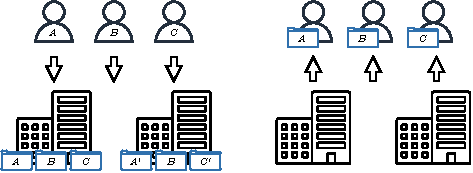
\includegraphics[height=0.6\textheight]{./assets/central_vs_decentral.drawio.pdf}
        \caption{Symbolbild: zentralisierte vs. dezentralisierte Datenspeicherung}
    \end{figure}
\end{frame}


\begin{frame}{Data Spaces III \footnotesize\cite{mollerIndustrialDataEcosystems2024}}
    \begin{columns}
        \begin{column}{0.6\textwidth}
            \begin{itemize}
                \item dezentralisierte Datenspeicherung\\
                      $\to$ verteilt \emph{by Design}, Datenredundanz
                
                \item Datenintegration auf semantische Ebene\\
                      $\to$ kein einheitliches Daten"=Schema notwendig
                
                \item Verschachtelung / Überlappung von Data Spaces\\
                      $\to$ \emph{Data Ecosystems}
                      % um einen oder mehrere föderierte Data Spaces
                      % technische Integration über Schnittstellen
                      % Datensouveränität & Verhinderung großer Daten-Silos: verschachtelt && überlappend
                
                \item Integration über Schnittstellen
                \item Erreichen gemeinsamer Ziele
            \end{itemize}
        \end{column}

        % \pause
        \begin{column}{0.4\textwidth}
            \begin{figure}
                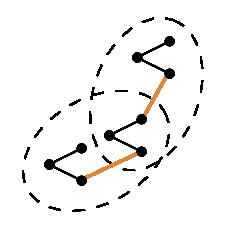
\includegraphics[height=0.5\textheight]{./assets/data_ecosystem_architecture.drawio.pdf}
                \caption{Data Ecosystem}
            \end{figure}
        \end{column}
    \end{columns}
\end{frame}


\begin{frame}{Data Spaces IV \footnotesize\cite{mollerIndustrialDataEcosystems2024}}
    \begin{itemize}
        \item flexible betriebliche Strukturen
        \item Zugang nur für bestimmte Akteure $\to$ \emph{Trusted Pool}
        \item sicheres, vertrauenswürdiges Data Sharing
        \item Einbettung in Data Ecosystem
        \item \emph{Data Space Member} vs. \emph{Data Ecosystem Party}
            % DSM: direkt technisch in DS eingebunden
            % DEP: nur indirekter Zugriff über Data Space Connector (Schnittstelle zu DSM)
        \item Governance"=Maßnahmen auf allen Abstraktionsebenen
            % Erfüllung rechtlicher Rahmenbedingungen
            % Ebene von DE, DS oder Use Case
    \end{itemize}
    
    % Data Spaces erfüllen am meisten Kriterien
    % Wie kann das funktionieren? $\to$ Social Linked Data
\end{frame}
